% \chapter{Experiments on the Real Robot}
\chapter{Real Robot Experiments}
\label{chap:ExperimentsOnARealRobot}
\minitoc


The second part of this work will focus towards a practical implementation of an open-source \ac{IL} approach on a real robotic system. The goal is to gain hands-on experience with the challenges and opportunities when setting up a connection to a real robot. This includes how to connect the robot with a workstation and how to control the robot from the workstation.
%  and what additional code is needed to adapt a model to our specific robot. 
The goal was to implement a simple and easy-to-use pipeline for robot communication, designed such that only the robot model needs to be replaced. 
% This includes a camera setup with calibration to capture the robot's environment and provide the necessary visual input for the model.
The overall setup is designed to be modular and extensible, enabling straightforward integration of different robot models and their respective software dependencies.
The full pipeline to setup and run a robot model on a robot is as follows:
\begin{enumerate}
    \item Setup Connection between PC and Robot. 
    \item Setup the control protocols, for controlling the Robot via PC (for example within a Python script~\cite{WelcomePythonorg2026}). There exists two different control protocols: 
    \begin{itemize}
        \item RTDE: Direct control Interface provided by Universal Robots~\cite{RealTimeDataExchange}.
        \item ROS 2: A popular high-level open-source framework for controlling different robots with the same Interface~\cite{ROS2Documentation}.
    \end{itemize}
    \item Camera Setup and Calibration.
    \item Implementing the robot model on the PC and adapt it to the UR5e.
    \item Testing the robot model and evaluating the performance.
\end{enumerate}

\paragraph{Robot Hardware}
For experiments, the UR5e Robot Arm~\cite{UserManualUR5e} from Universal Robots will be used, see \autoref{fig:UR5eRobotAmberg}. 
It is a collaborative robot (cobot) designed for safe human-robot interaction. The UR5e provides a versatile and user-friendly 12 inch touchscreen interface for controlling and static programming the robot. The Gripper 2F-140 from Robotiq was used, which has a payload of 2.5 kg and a stroke of 10 to 125 Newton~\cite{AdaptiveGrippersRobotiq}. 

\begin{figure}[!ht]
	\centering
	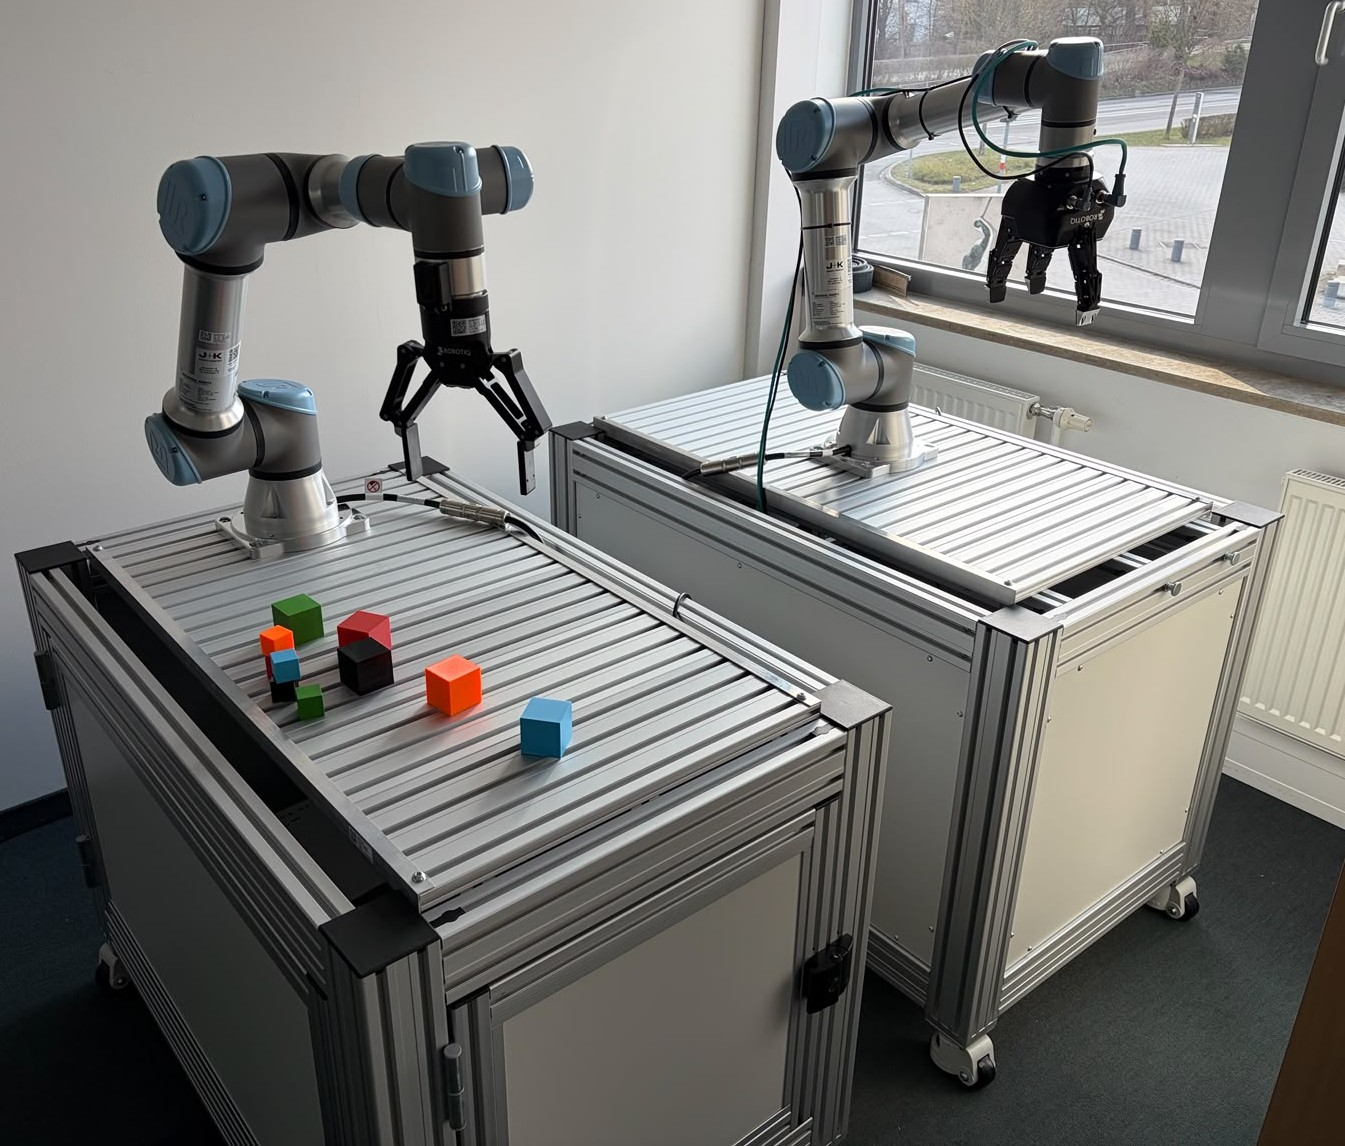
\includegraphics[width=0.6\linewidth]{./chapter9/media/UR5eRobotAmberg.jpeg}
	\caption[UR5e Robot from Universal Robots]{UR5e Robot from Universal Robots: This UR5e robot was used for experiments.}
	\label{fig:UR5eRobotAmberg}
\end{figure}


In~\autoref{tab:UR5eSpecifications} some specifications of the Robot are listed. 
\begin{table}[h]
    \centering
    \renewcommand{\arraystretch}{1.3}
    
    \begin{tabular}{|>{\raggedright\arraybackslash}m{4.6cm}|>{\raggedright\arraybackslash}m{4.3cm}|}
        \hline
        \rowcolor{blue!10}
        \multicolumn{2}{|>{\centering\arraybackslash}m{9.5cm}|}{\rule{0pt}{3ex}\textbf{Robot:} UR5e Robot Arm from Universal Robots\vspace{1ex}} \\
        \hline
        Degrees of freedom & 6 rotating joints \\
        \hline
        Joints speed & 180°/s \\
        \hline
        Payload & 5 kg  \\
        \hline
        Reach & 850 mm \\
        \hline
        Weight & 12 kg \\
        \hline
        Materials & Powder coated steel \\
        \hline
    \end{tabular}
    \caption{Specifications of the UR5e Robot Arm. Source:~\cite{UR5e_2}}
    \label{tab:UR5eSpecifications}
\end{table}




\section{Establishing PC-to-Robot Connectivity}
Many modern robot learning models require substantial computational resources for image processing, perception and action generation. In particular, many \ac{VLA} models rely on high-performance GPUs, such as an NVIDIA RTX 4090, to achieve (near) real-time inference. 
Due to these computational requirements, the robot model must be deployed on an external workstation, rather than directly on the UR5e robot, whose onboard hardware is not designed for executing large-scale deep learning models. In addition, some extra software is needed for running a robot model and communicating with the robot control interface, which can be easily installed on a PC. Consequently, a communication connection between the workstation and the robot had to be established, which enables the external computer to execute the robot model, send motion commands to the robot or receive sensor and state information from the robot required for closed-loop control.

To facilitate this process, a detailed \textit{setup guide} was created that documents the individual steps required to establish a reliable connection.
% between the workstation and the UR5e robot. 
The guide covers the configuration of network settings and communication ports on both devices, procedures for verifying network connectivity, the activation of Remote Control mode and required services on the robot, as well as the configuration of the External Control functionality. This includes the creation of an External Control program that must be executed on the robot before control commands can be transmitted from the workstation.






\section{Robot Control Protocols}


\subsection{ROS 2 - Robot Operating System 2}
ROS 2 (Robot Operating System 2)~\cite{ROS2Documentation} is an open-source robotics middleware framework used for building modular and distributed robotic systems. It organizes software into independent components called nodes, where each node performs a specific function such as perception, control, or planning. These nodes communicate with each other using standardized interfaces.
% , including topics, services and actions. 
ROS 2 provides the communication infrastructure that enables reliable data exchange between different parts of a robotic system. In this way, it acts as the “plumbing” layer that connects sensing, computation and actuation in robotics applications. A key advantage of ROS 2 is that it allows the same software components to be reused across different robotic platforms without requiring changes to the core code, as long as the robots support the same ROS 2 communication interfaces.
The complete ROS 2 implementation developed during this work is publicly available in the following repository:
\begin{center}
    \url{https://github.com/sweidner2001/RobotUR5e_ROS2}
\end{center}
% The complete ROS2 Repository is available under: \url{https://github.com/sweidner2001/RobotUR5e_ROS2}

The repository contains scripts and configuration files required to establish communication with the UR5e robot and to launch the corresponding ROS 2 nodes. These scripts automate the initialization process and provide a easy-to-use setup for robot control, visualization and simulation.
The ROS 2 environment integrates several commonly used robotics tools:
\begin{itemize}
    \item \textbf{RViz}~\cite{RvizMainPage} is a 3D real-time visualization tool for ROS, see~\autoref{fig:RViz}. It provides a view of the robot model, sensors and other information in a 3D space. It can be used to display sensor data from robots, such as point clouds, camera images, robot trajectories. While RViz can be used in conjunction with Gazebo, it is not a simulation environment of itself.

    \item \textbf{MoveIt}~\cite{MoveIt2Documentationa} is a motion planning framework for robotic manipulators that computes collision-free trajectory generation and collision checking between start and target poses, see~\autoref{fig:MoveIt}. It can be used for both simulated and real robotic systems.
    
    \item \textbf{Gazebo}~\cite{Gazebo} is a physics-based simulation environment commonly used in conjunction with ROS 2 and RViz. It enables realistic simulation of robot dynamics (mass, inertia, gravity), sensors (cameras, lidar, force sensors) and the environment (collisions, friction). Gazebo provided a virtual testing environment for validating robot configurations and control algorithms before deployment on the physical UR5e robot.
\end{itemize}

\begin{figure}[!ht]
    \centering
    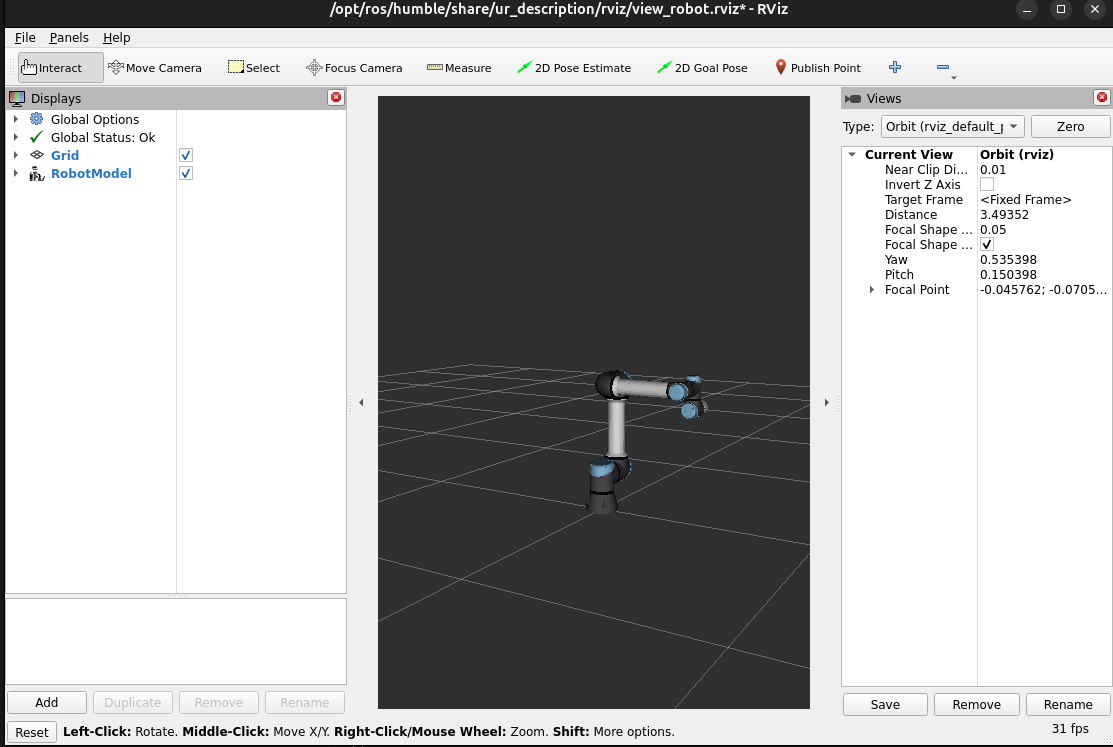
\includegraphics[width=0.8\linewidth]{./chapter9/media/Rviz}
    \caption[RViz: Visualization Tool]{RViz is a 3D real-time visualization tool used in ROS 2.}
    \label{fig:RViz}
\end{figure}
\begin{figure}[!ht]
    \centering
    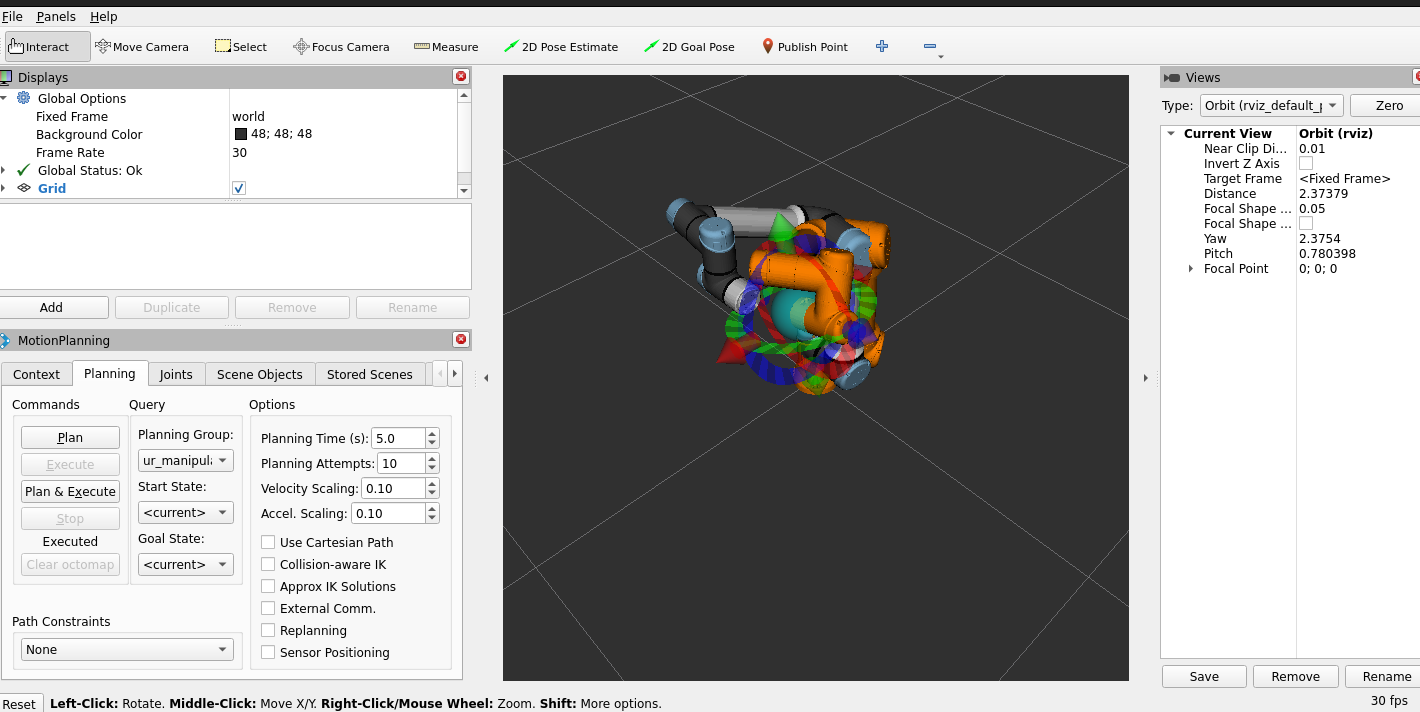
\includegraphics[width=0.8\linewidth]{./chapter9/media/RvizWithMoviIt}
    \caption[MoveIt: Motion Planning Tool]{MoveIt is a motion planning framework and here used together with RViz. The orange robot represent the target pose of the robot and within the RViz you can simulate the trajectory, which is planned by MoveIt.}
    \label{fig:MoveIt}
\end{figure}

In addition to the software implementation, comprehensive documentation was created to support the deployment of a robot model via ROS 2. The documentation describes the procedures required to establish communication with the robot via ROS 2, set the UR5e robot in External Control mode, ROS 2 commands to control the robot and commands for troubleshooting. Furthermore it explains the usage of the provided scripts and workflows for controlling the robot within both simulated and real-world environments.


\paragraph{Setup}
To simplify the development and deployment process, the ROS 2 project was implemented using a Dev Container environment~\cite{DevelopingContainer}. This approach provides an isolated and reproducible software environment, eliminating the need to install ROS 2, robot drivers and additional dependencies directly on the host system. As a result, all developers can work within a consistent environment while avoiding dependency conflicts and configuration issues.
The Dev Container provides a fully configured ROS 2 workspace tailored for Universal Robots development. It includes the required communication interfaces for the UR5e robot, as well as commonly used robotics tools such as Gazebo, MoveIt and RViz.
The Dev Container setup follows a layered workflow consisting of four main components:
\begin{enumerate}
    \item \textbf{devcontainer.json:} Defines the configuration for the development container, including user settings, mounted directories, environment variables, Visual Studio Code extensions and post-creation commands. It serves as the entry point for building and configuring the container environment.
    \item \textbf{Dockerfile:} Defines the base development environment and installs all required software packages, including the ROS 2 Distribution, the Universal Robots driver, Gazebo, RViz and MoveIt. 
    During the image build process, the script \texttt{setup\_workspace\_additional.sh} is executed. 
    \item \textbf{setup\_workspace\_additional.sh:} This script contains permanent configuration steps that become part of the Docker image and are therefore available in every container instance created from the image. You can add easily your additional setup here to extend the docker image without editing the base Dockerfile.
    \item \textbf{setup\_workspace\_temp.sh:} After the Docker image has been built successfully, the \texttt{devcontainer.json} configuration executes the script \texttt{setup\_workspace\_temp.sh}. In contrast to the permanent setup script, this script is executed each time a new container instance is created. It is intended for temporary workspace configuration, experimental package installations and project-specific modifications that should not require rebuilding the entire Docker image. 
\end{enumerate}
This separation between permanent and temporary configuration steps provides a flexible and fast development workflow while maintaining a stable and reproducible base environment.


\paragraph{Provided Scripts}
See~\autoref{tab:launch_scripts} for an overview of the provided easy-to-use launch scripts.
\begin{table}[!h]
    \centering
    \renewcommand{\arraystretch}{1.5}
    \begin{tabular}{|>{\raggedright\arraybackslash}p{4.5cm}|>{\raggedright\arraybackslash}p{10.5cm}|}
        \hline
        \rowcolor{blue!10}
        \textbf{Script Name} & \textbf{Description} \\
        \hline
        \texttt{launch\_std.sh} & Launches the UR robot driver to connect to a real UR robot. This allows for direct control of the robot through ROS 2 topics and services. If the command is successful, RViz should start and shows the robot in its current pose. If the robot is not visible, there is a connection error. \\
        \hline
        \texttt{launch\_RViz\_MoveIt.sh} & Launches the UR robot driver together with MoveIt and RViz. This allows controlling the real robot via the MoveIt planning interface in RViz. \\
        \hline
        \texttt{sim\_launch\_RViz\allowbreak\_Gazebo.sh} & Launches the UR5e simulation in Gazebo with RViz. The robot is simulated and can be visualized via RViz. \\
        \hline
        \texttt{sim\_launch\_RViz\allowbreak\_MoveIt\allowbreak\_Gazebo.sh} & Launches the UR5e simulation in Gazebo with MoveIt and RViz. In addition to the simulation, MoveIt is loaded, enabling motion planning within the simulation. \\
        \hline
    \end{tabular}
    \caption{Launch Scripts for UR5e Robot Control}
    \label{tab:launch_scripts}
\end{table}


\paragraph{Gripper Control}
To control the gripper, additional ROS 2 packages and interfaces are required, as the gripper is not directly controlled through the main robot driver. Due to missing instructions, how to control the gripper directly with a ROS 2 Node, the gripper wasn't finished implemented and is not functional yet. Some additional specific \texttt{urdf.xacro} files are needed, to connect the gripper to the robot model in Rviz. However, the ROS 2 setup provides the necessary infrastructure to integrate gripper control in the future.


\paragraph{Summary}
In summary, the ROS 2 implementation provides a comprehensive framework for controlling the UR5e robot arm from an external workstation, but there was some difficultness with the gripper control, which is not yet implemented. For this reason, the decision was made to prioritise the implementation of the RTDE interface provided by Universal Robots, as ready-made Python packages~\cite{WelcomePythonorg2026} were already available for this purpose. 
% The aim was to implement an initial working robot model as quickly as possible.






\subsection{RTDE - Real-Time Data Exchange}
RTDE (Real-Time Data Exchange)~\cite{RealTimeDataExchange} is a direct communication interface provided by Universal Robots for exchanging data between an external computer and the robot controller. It enables fast, low-latency transmission of sensor data and control commands. Compared to ROS 2, RTDE operates closer to the hardware and therefore provides higher update rates. This makes it suitable for real-time robot applications in the Universal Robots universe, where fast and reliable data exchange is required. The advantage is that RTDE is easy to set up. However, the disadvantage is that the interface must be adapted when switching to a different robot.
The complete RTDE implementation developed during this work is publicly available in the following repository:
\begin{center}
    \url{https://github.com/sweidner2001/RobotUR5e_RTDE}
\end{center}





\paragraph{Provided Scripts}
Some test scripts are provided, for example a static pick-and-place demo with three cubes, which are stacked on top and another script for the reverse process. The scripts demonstrate how to use the RTDE interface to control the robot's movement and gripper, as well as how to read sensor data from the robot. The provided code serves as a starting point for implementing more complex robot control algorithms and can be easily extended to include additional functionality or to adapt to different robotic tasks. 



\paragraph{Setup}
To simplify development and deployment, the RTDE project was implemented in a dedicated Python virtual \texttt{venv}-environment~\cite{VenvCreationVirtual}. This approach provides an isolated and reproducible setup that can be executed on any system with Python installed, while avoiding dependency conflicts with globally installed packages.

The environment can be easily set up by executing the \texttt{setup.sh} script, which automatically creates the virtual environment and installs all required dependencies for working with the RTDE interface. In addition, the script configures the project structure such that Python modules can be imported using absolute paths relative to the project root. All project scripts on every location in the project structure can be conveniently executed from within Visual Studio Code using the ``run button'' functionality, with all imports resolving correctly once the environment is activated.


\paragraph{Summary}
% The project includes several example scripts for testing and demonstration purposes. One example implements a static pick-and-place scenario in which three cubes are stacked in a predefined order, while another script performs the reverse operation.
The Project demonstrates how the RTDE interface can be used to control robot motion and gripper actions, as well as how to access and process sensor data from the robot and serves as a starting point for more advanced robot control strategies. 
% They are designed to be easily extensible, allowing additional functionality to be integrated or adapted to different manipulation tasks.




\section{Summary}
Overall, the robot setup required a significant amount of time, in particular the ROS 2 implementation, which ultimately remained incomplete and did not always operate reliably. However, by using the RTDE interface, it was still possible to quickly run a simple static pick-and-place demonstration on the UR5e robot.

Due to the limited scope of this thesis, no complete robot learning model was deployed on the UR5e, and the focus was placed on developing the foundational robot setup required for future deployment of robot learning models on the UR5e.
Nevertheless, initial considerations were made regarding the placement of cameras around and on the robot. A suitable 3D model for a camera mount on the robot was also identified for potential 3D printing.
In addition, an overview of ten promising open-source robot learning models was created, which are expected to be implemented with low integration effort in future works.






\chapter{Thesis Resumé}
\minitoc
This chapter concludes the thesis by synthesizing the key findings on video-based imitation learning for robotics and identifying promising directions for future work in advancing general-purpose robotic intelligence.

\section{Summary}

This thesis investigates imitation learning as a promising approach for enabling robots to acquire complex skills from demonstrations, with the long-term goal of general-purpose robotic intelligence.
It first introduces fundamental concepts in machine learning and robotics, with a focus on the data requirements for training generalist robotic systems and the principles how robots can be instructed to perform desired tasks. Building on this foundation, the thesis examines the paradigm of \ac{LfV}, addressing how relevant knowledge can be extracted from large-scale internet video data and transferred to robotic systems for policy learning and control. In particular, it highlights the importance of robust video understanding for interpreting human demonstrations in imitation learning settings.
Subsequently, different approaches for learning robot policies from video data are discussed, including representation learning methods, reinforcement learning-based and imitation learning approaches, hybrid techniques, and large-scale vision-language-action models. The thesis further analyzes key challenges and future research directions, emphasizing the gap between current methods and the goal of general-purpose robotic intelligence. Emerging paradigms such as diffusion-based policies, world models, and causally aware learning systems are identified as promising directions for improving generalization, reasoning, and adaptability in robotic agents.

For practical insights, selected imitation learning approaches deployed on real robotic systems are examined. In addition, a basic robotic setup for a UR5e robot arm from Universal Robots was implemented, providing a foundational platform for future experiments with robot learning models.

Overall, the thesis provides a structured overview of imitation learning and video-based robotic learning, connecting theoretical foundations with practical implementation aspects.




\section{Outlook}

This thesis provided an overview of imitation learning and video-based robot learning, as well as the practical foundations required for deploying learning-based approaches on a real UR5e robot.
The most immediate next step is the deployment and evaluation of a robot learning model on the real UR5e robot, to gain practical insights into real-world deployment and the challenges that arise in this context.
Future work should therefore focus on adapting and deploying one of the identified open-source robot models to the UR5e robot.
% , which includes writing a control script for the robot with the RTDE interface and integrating a camera system for perception of the robot. If this works, the ROS 2 implementation can be further developed and tested, to provide a more flexible and modular framework for robot control.
This process includes the implementation of a robust control pipeline using the RTDE interface, the integration of a camera system for visual perception and the development of data-processing pipelines for model inference. Once a complete perception-to-action pipeline is operational, the existing ROS 2 implementation can be further developed and tested to provide a more modular and extensible framework for robot control, simulation and experimentation.

\paragraph{Techniques \& Architectures}
Beyond the practical implementation, several research directions in robot learning remain promising. Recent architectures such as TimeSformers, Q-Formers, Action Chunking Transformers, Conditional Behavior Transformers (C-BeT) and Conditional Variational Autoencoders (C-VAE) could be investigated for their applicability to robotic policy learning. 
Additional research could investigate meta-learning approaches that allow robots to rapidly adapt to new tasks with minimal additional training. The combination of world models, causal reasoning and multimodal foundation models may represent a crucial step toward the development of more general-purpose robotic agents. The advantages and disadvantages of monolithic and compositional models can be worked out too.

Furthermore, combining traditional physics-based simulation with video prediction models represents an interesting avenue for future work. Such hybrid simulators could improve planning capabilities while maintaining physical consistency.

Another promising direction is the application of Video Question Answering (VQA) techniques to robotics. Robot systems could query video understanding models with questions such as ``Was the task completed successfully?'' to automatically generate supervision signals and evaluate task execution. While VQA has been widely used with images, but not with videos as input.



\paragraph{Learning from Videos}
An underexplored area is the use of \ac{LfV} rewards to augment offline reinforcement learning datasets. For example, an LfV policy could be refined through online reinforcement learning while using video-derived rewards to guide optimization.

As \ac{LfV} continues to gain importance, several open research questions remain. One challenge is the recovery of action information from action-free video demonstrations. Future work could systematically compare existing action representations $\hat{a} \in \hat{A}$ and evaluate their effectiveness for transferring knowledge from videos to robotic policies. Additionally, novel action representations could be developed that combine the strengths of existing approaches while reducing ambiguity during policy learning.




\paragraph{Datasets, Benchmarks and Evaluation}
Future work could also focus on the systematic analysis of existing robotics datasets and their coverage of tasks, environments and manipulation skills. Video editing and synthetic data generation techniques may provide opportunities to augment existing datasets and improve their diversity.

Finally, progress in Learning from Videos requires improved benchmark suites and evaluation metrics. Current benchmarks often focus primarily on task success rates, while future evaluations should also measure generalization, robustness, data efficiency, sim-to-real transfer performance and causal understanding. The development of such benchmarks will be crucial for the quantitative assessment of the performance of robot models and will set the future direction for research.


\paragraph{Summary}
Overall, the rapid progress in robot learning and the complementary fields of \acp{LLM} and vision models suggests that robot learning will remain a highly active research area in the coming years. Continued advances in these fields may ultimately contribute to the development of robotic systems capable of learning, adapting and generalizing across a wide range of real-world tasks.































